\documentclass[tikz,border=5pt]{standalone}
\usepackage{ctex,amsmath}
\usetikzlibrary{arrows.meta,calc}
\tikzset{>=Latex,axis/.style={gray,->},water/.style={blue!65!black},force/.style={orange!85!black,thick,->}}
\begin{document}
\begin{tikzpicture}[font=\small]
\fill[blue!8](-.85,0)--plot[domain=0:4,samples=80] ({-.85*(1+\x)^(-.25)},-\x)
--plot[domain=4:0,samples=80] ({.85*(1+\x)^(-.25)},-\x)--cycle;
\draw[water,thick]plot[domain=0:4,samples=80] ({-.85*(1+\x)^(-.25)},-\x);
\draw[water,thick]plot[domain=0:4,samples=80] ({.85*(1+\x)^(-.25)},-\x);
\draw[water] (0,0)ellipse[x radius=.85,y radius=.14];
\draw[water] (0,-3)ellipse[x radius=.601,y radius=.11];
\draw[gray,dashed](0,.4)--(0,-4.3);
\draw[<->](0,.48)--(.85,.48)node[midway,above]{$r_0$};
\draw[gray,dashed](.85,.12)--(.85,.60);
\draw[<->](0,-3.35)--(.601,-3.35)node[midway,below]{$r(y)$};
\draw[water,thick,->](-1.28,0)--(-1.28,-.7)node[midway,left]{$v_0$};
\draw[water,thick,->](-1.28,-2.7)--(-1.28,-3.7)node[midway,left]{$v(y)$};
\draw[axis](1.60,.12)--(1.60,-4.3)node[below]{$y$};
\draw[gray,dashed](.90,0)--(1.67,0)node[right]{$0$};
\draw[gray,dashed](.64,-3)--(1.67,-3)node[right]{$y$};
\node[above]at(-.6,.78){出口};
\end{tikzpicture}
\begin{tikzpicture}[font=\small]
\begin{scope}[xshift=-2.6cm]
\fill[blue!7](-.85,1.2)--(-.85,-1.2)arc[start angle=180,end angle=360,x radius=.85,y radius=.16]--(.85,1.2)--cycle;
\draw[water](-.85,1.2)--(-.85,-1.2)(.85,1.2)--(.85,-1.2);
\draw[water](0,1.2)ellipse[x radius=.85,y radius=.16];
\draw[water](-.85,-1.2)arc[start angle=180,end angle=360,x radius=.85,y radius=.16];
\draw[water,dashed](-.85,-1.2)arc[start angle=180,end angle=0,x radius=.85,y radius=.16];
\draw[gray,dashed](0,1.2)--(0,-1.2);
\draw[->](0,1.2)--(.85,1.2)node[midway,above]{$r$};
\draw[<->](-1.15,-1.2)--(-1.15,1.2)node[midway,left]{$\mathrm ds$};
\node[above]at(0,1.7){局部圆柱};
\end{scope}
\begin{scope}[xshift=1.5cm]
\fill[blue!7](1,0)arc[start angle=0,end angle=180,radius=1]--cycle;
\draw[water,thick](1,0)arc[start angle=0,end angle=180,radius=1];
\draw[gray,thick](-1,0)--(1,0);
\draw[force](0,.08)--(0,.75);
\node[above]at(0,1.10){$\Delta p\,2r\,\mathrm ds$};
\draw[force](-1,0)--(-1,-.75)node[left]{$\sigma\,\mathrm ds$};
\draw[force](1,0)--(1,-.75)node[right]{$\sigma\,\mathrm ds$};
\draw[<->](-1,-1.12)--(1,-1.12)node[midway,below]{$2r$};
\node[above]at(0,1.7){上半圆柱横截面};
\end{scope}
\end{tikzpicture}
\begin{tikzpicture}[font=\small,x=.70cm,y=4.5cm]
\draw[axis](0,.50)--(8.7,.50)node[right]{$z$};
\draw[axis](0,.50)--(0,1.12)node[above]{$r/r_0$};
\foreach \t in {0,2,4,6,8}\draw[gray](\t,.50)--(\t,.49)node[below]{$\t$};
\foreach \t in {.6,.8,1.0}\draw[gray](0,\t)--(-.08,\t)node[left]{$\t$};
\draw[water,very thick]plot[domain=0:8,samples=101] (\x,{(1+\x)^(-.25)});
\draw[orange!85!black,very thick] plot coordinates {(0.000000,1.000000000) (0.080000,0.982562253) (0.160000,0.966477847) (0.240000,0.951572339) (0.320000,0.937701650) (0.400000,0.924745547) (0.480000,0.912602780) (0.560000,0.901187361) (0.640000,0.890425720) (0.720000,0.880254468) (0.800000,0.870618644) (0.880000,0.861470318) (0.960000,0.852767465) (1.040000,0.844473056) (1.120000,0.836554309) (1.200000,0.828982082) (1.280000,0.821730365) (1.360000,0.814775852) (1.440000,0.808097591) (1.520000,0.801676682) (1.600000,0.795496023) (1.680000,0.789540097) (1.760000,0.783794780) (1.840000,0.778247191) (1.920000,0.772885546) (2.000000,0.767699042) (2.080000,0.762677756) (2.160000,0.757812550) (2.240000,0.753094994) (2.320000,0.748517298) (2.400000,0.744072246) (2.480000,0.739753146) (2.560000,0.735553779) (2.640000,0.731468357) (2.720000,0.727491488) (2.800000,0.723618135) (2.880000,0.719843593) (2.960000,0.716163457) (3.040000,0.712573598) (3.120000,0.709070141) (3.200000,0.705649448) (3.280000,0.702308094) (3.360000,0.699042856) (3.440000,0.695850695) (3.520000,0.692728743) (3.600000,0.689674292) (3.680000,0.686684781) (3.760000,0.683757785) (3.840000,0.680891010) (3.920000,0.678082279) (4.000000,0.675329526) (4.080000,0.672630790) (4.160000,0.669984207) (4.240000,0.667388005) (4.320000,0.664840495) (4.400000,0.662340070) (4.480000,0.659885198) (4.560000,0.657474418) (4.640000,0.655106334) (4.720000,0.652779613) (4.800000,0.650492983) (4.880000,0.648245225) (4.960000,0.646035174) (5.040000,0.643861715) (5.120000,0.641723777) (5.200000,0.639620337) (5.280000,0.637550413) (5.360000,0.635513060) (5.440000,0.633507375) (5.520000,0.631532487) (5.600000,0.629587562) (5.680000,0.627671795) (5.760000,0.625784415) (5.840000,0.623924677) (5.920000,0.622091867) (6.000000,0.620285294) (6.080000,0.618504294) (6.160000,0.616748227) (6.240000,0.615016475) (6.320000,0.613308442) (6.400000,0.611623554) (6.480000,0.609961255) (6.560000,0.608321009) (6.640000,0.606702298) (6.720000,0.605104622) (6.800000,0.603527495) (6.880000,0.601970450) (6.960000,0.600433033) (7.040000,0.598914807) (7.120000,0.597415347) (7.200000,0.595934241) (7.280000,0.594471091) (7.360000,0.593025512) (7.440000,0.591597128) (7.520000,0.590185578) (7.600000,0.588790509) (7.680000,0.587411581) (7.760000,0.586048461) (7.840000,0.584700828) (7.920000,0.583368370) (8.000000,0.582050784)};

\draw[water,very thick](3,1.055)--(3.8,1.055)node[right,black]{无表面张力};
\draw[orange!85!black,very thick](3,.96)--(3.8,.96)node[right,black]{$\eta=0.4$};
\end{tikzpicture}
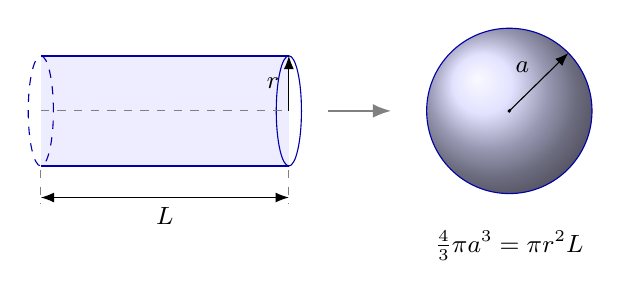
\begin{tikzpicture}[font=\small]
\fill[blue!7](0,.7)--(3.15,.7)--(3.15,-.7)--(0,-.7)--cycle;
\draw[water,thick](0,.7)--(3.15,.7)(0,-.7)--(3.15,-.7);
\draw[water,dashed](0,0)ellipse[x radius=.16,y radius=.7];
\draw[water](3.15,0)ellipse[x radius=.16,y radius=.7];
\draw[gray,dashed](0,0)--(3.15,0);
\draw[->](3.15,0)--(3.15,.7)node[midway,left]{$r$};
\draw[<->](0,-1.10)--(3.15,-1.10)node[midway,below]{$L$};
\draw[gray,dashed](0,-.75)--(0,-1.18)(3.15,-.75)--(3.15,-1.18);
\draw[gray,thick,->](3.65,0)--(4.45,0);
\shade[ball color=blue!15](5.95,0)circle[radius=1.05];
\draw[water](5.95,0)circle[radius=1.05];
\fill(5.95,0)circle[radius=.025];
\draw[->](5.95,0)--(6.70,.735)node[midway,above left]{$a$};
\node[below]at(5.95,-1.40){$\frac43\pi a^3=\pi r^2L$};
\end{tikzpicture}
\end{document}
